\documentclass[12pt]{article}
\usepackage{graphicx,epsfig,palatino,epstopdf}


\title{Lab 2: PF}
\author{
        Miquel Marti Rabadan\\
        miquelmr@kth.se
}
\date{\today}



\begin{document}
\maketitle


\section{PART I - Preparatory Questions}

\subsection*{Particle Filters:}

\paragraph{1 - What are the particles of the particle filter?} 
Particles are samples drawn from the posterior distribution used to represent this distribution with a finite number of points.

\paragraph{2 - What are importance weights, target distribution, and proposal distribution and what is the relation between them?}
The importance weight is the probability of having a measurement given we are in a state. Target distribution is the true posterior from which we want to draw the particles and proposal distribution is our sampled distribution. The importance weights are used to adjust the later so it approaches the target distribution.

\paragraph{3 - What is the cause of particle deprivation and what is the danger}
Particle deprivation means having no particles where the state has actually some probability of being. This most likely occurs when performing the estimation in a high-dimensional space and having a number of particles too small to cover all relevant regions with high likelihood. However, it can eventually occur as a result of the random re-sampling step where the importance factor is used to sample from the intermediate distribution, though the probability of that happening is exponentially small with the number of particles (but non-zero).

\paragraph{4 - Why do we resample instead of simply maintaining a weight for each particle always.}
We re-sample because maintaining a weight for each particle  would approximate the posterior but would lead many of the particles to regions of low posterior probability so many more particles would be needed to have a good representation, depending on the shape of the true posterior.

\paragraph{5 - Give some examples of the situations which the average of the particle set is not a good representation of the particle set.}
In particle distributions with peaks the average would be no representative. In the extreme case of only two peaks of same density, the average would fall in the middle, which is not a good representation at all.

\paragraph{6 - How can we make inferences about states that lie between particles.}
Assuming continuity between number of particles across adjacent states and interpolating between the number of particles of the states around or using Gaussian kernels around the particles so the density function becomes continuous, as a discrete sum of continuous functions.


\paragraph{7 - How can sample variance cause problems and what are two remedies?}
Sampling variance is the difference between the particle distribution and the target distribution, so the error between it. It can be reduced using more particles. Two methods to reduce the variance are delayed re-sampling, keeping the importance weights as part of the description and re-sampling less frequently with the compound weight, and low variance sampling, in which samples are not selected independently but also related to a single random number computed for all samples taken at a step and proportional to the weight.

\paragraph{8 - For robot localization for a given quality of posterior approximation, how are the pose uncertainty (spread of the true posteriori) and number of particles we chose to use related.}
The more spread the true posteriori is, the bigger the number of particles.



\section{PART II - Matlab Exercises}
\subsection{Warm up problem with the Particle Filter}

\paragraph{1 - What are the advantages/drawbacks of using the 2D State Space model (6) compared to the 3D (8) for the target moving on a line? Motivate.}
Using (6) we have a simpler model in which the angle is defined by a constant value, while in (8) the angle is part of the state so it is conditioned to errors in its estimation. The later though can be used as well to define more complex models representing more complex movements changing only the control sequence.

\paragraph{2 - What types of circular motions can we model using (9)? What are the limitations (what do we need to know/fix in advance)?}
With (9) we can model circular movements with constant linear and angular velocities which have to be known/fixed beforehand.

\paragraph{3 - What is the purpose of keeping the constant part in the denominator of (10)?}
The constant part in the denominator is kept for normalization purposes.

\paragraph{4 - How many random numbers do you need to generate for the Multinomial re-sampling method? How many do you need for the Systematic re-sampling method?}
For the Multinomial re-sampling you need to generate M different random numbers while for the Systematic version only one.

\paragraph{5 - With what probability does a particle with weight \(\omega=\frac{1}{M}+\epsilon\) survive the re-sampling step in each type of re-sampling (vanilla and systematic)? What is this probability for a particle with \(0\leq \omega < \frac{1}{M} \)? What does this tell you? (Hint: it is easier to reason about the probability
of not surviving, that is M failed binary selections for vanilla, and then subtract that amount from 1.0 to find the probability of surviving. } For the vanilla re-sampling a particle is drawn with probability \(\omega\). The probability of it surviving is the probability of being drawn in at least one of the M chances. It is easier to derive the complementary probability, that is the probability of not being drawn in any of the M chances \((1-\omega)^M\). The survivability probability is then \(1-(1-\omega)^M\), it is the same for both cases. For the systematic re-sampling, with the first case, the survivability probability is 1, because the particles form a set of bins and at each iteration the value added to the random number is \(\frac{1}{M}\) so the particle selection always includes at least once the particles with weight greater than the separation, as is the case for \(\omega = \frac{1}{M}+\epsilon\). For the other case, the probability of surviving is proportional both to the weight of the particle and to the number of particles being drawn M. In the limit where \(omega=\frac{1}{M}\), the probability of being drawn would be 1, so the proportionality factor has to be M and the survivability probability is \(M\omega\).

\paragraph{6 - Which variables model the measurement noise/process noise models?}
The measurement noise is modelled by variable \texttt{Sigma\_Q} and the process noise by \texttt{Sigma\_R}.

\paragraph{7 - What happens when you do not perform the diffusion step?(You can set the process noise to 0)} After a few re-samplings only one particle survives, all the others converge to this one, the one with highest weight, in the case of the fixed motion the one closer to the true state in the initial uniform distribution of the particles.

\paragraph{8 - What happens when you do not re-sample? (set RESAMPLE MODE=0)} The initial uniform distribution across the space does not change. The particles move according to the motion model and the process noise and the weights might be updated due to different measurements but they are not used for the re-sampling so the distribution remains just the same and does not converge to the real state.

\paragraph{9 - What happens when you increase/decrease the standard deviations(diagonal elements of the covariance matrix) of the observation noise model? (try values between 0.0001 and 10000)}
For small values the particle cloud does not converge to the true value as the measurements are expected to be very accurate and they are not so are classified as outliers and the weights are set uniformly. For a value of 10, this happens for a while until a measurement is seen as good (inside the likelihood threshold) and then it converges immediately.

\paragraph{10 - What happens when you increase/decrease the standard deviations(diagonal elements of the covariance matrix) of the process noise model? (try values between 0.0001 and 10000)}
For small values, the particles are very concentrated on a single point which depends on the initial distribution and slowly converge to the true state. For high values, the convergence is fast but the variance is high and the particles are very spread around the true state point.

\paragraph{11 - How does the choice of the motion model affect a reasonable choice of process noise model?}
The process noise model choice will depend on the motion model, if the model used in the prediction does not correspond exactly to the true one, more noise can compensate for that as the spread of the particle cloud will be bigger. If in this case the noise is too small, it will fail to track.

\paragraph{12 - How does the choice of the motion model affect the precision/accuracy of the results? How does it change the number of particles you need?}
A motion model that is not the correct one will need of a greater process noise to keep track and thus the use of a more spread particle cloud which will require more particles.

\paragraph{13 - What do you think you can do to detect the outliers in third type of measurements? Hint: what happens to the likelihoods of the observation when it is far away from what the filter has predicted?}
Setting a threshold for the mean likelihood of the measurement given the state, if it is too low it can be assumed to be an outlier. 

\paragraph{14 - Using 1000 particles, what is the best precision you get for the second type of measurements of the object moving on the circle when modelling a fixed, a linear or a circular motion(using the best parameter setting)? How sensitive is the filter to the correct choice of the parameters for each type of motion?}
For both the linear and the circular motion models low values for the process noise can be used but for the fixed motion the process noise has to be much bigger to compensate. Linear and circular motion models have small differences but still the circular motion gives smaller error as one would expect. The lowest errors and the parameters are shown in Table \ref{q14}. When choosing the parameters, for big enough values of Q, the estimation is more sensitive on the value of R, and more clearly in the fixed motion model.

\begin{table}[]
\centering
\caption{Estimation error for the best combination of parameters trying to estimate the circular movement of an object with different motion models.}
\label{q14}
\begin{tabular}{ccc|c}
\textbf{Motion model} & \textbf{\texttt{Sim\_Q}} & \textbf{\texttt{Sim\_R}} & \textbf{Estimation error} \\ \hline
\textit{Fixed}        & 300                          & 50                       & \(11.9 \pm 6.3 \)              \\
\textit{Linear}       & 300                          & 5                        & \( 7.5 \pm 4.0     \)           \\
\textit{Circular}     & 300                          & 3                        & \(7.4 \pm 3.8\)               
\end{tabular}
\end{table}

\subsection{Main problem: Monte Carlo Localization}

\paragraph{15 - What parameters affect the mentioned outlier detection approach? What will be the result of the mentioned method if you model a very weak measurement noise \(|Q| \to 0\)?}
The threshold selected and the measurement noise model assumed. A very weak measurement noise will result in classifying all the measurements as outliers as for smaller Q the likelihood function would have a very narrow peak around the measurement and thus being it very easy that the likelihood falls beyond the threshold.

\paragraph{16 - What happens to the weight of the particles if you do not detect outliers?}
If an outlier measurement is not detected the weights of the particles closer to the outlier are given a much greater value thus giving an erroneous set of particles after the next re-sampling.

\subsection{Results}

\subsubsection{\texttt{map\_sym2+so\_sym2\_nk}}

In the first map, when performing a tracking task the particle filter performs well because knows where to initialize the particles. Conversely, the localisation when no initial pose has been set is very unlikely to be right due to the symmetries on the two axis leading to four possible hypotheses which are equally likely, one close to each landmark. Figure \ref{fig:track} shows the result for the tracking task.\\

\begin{figure}[htp]

\centering
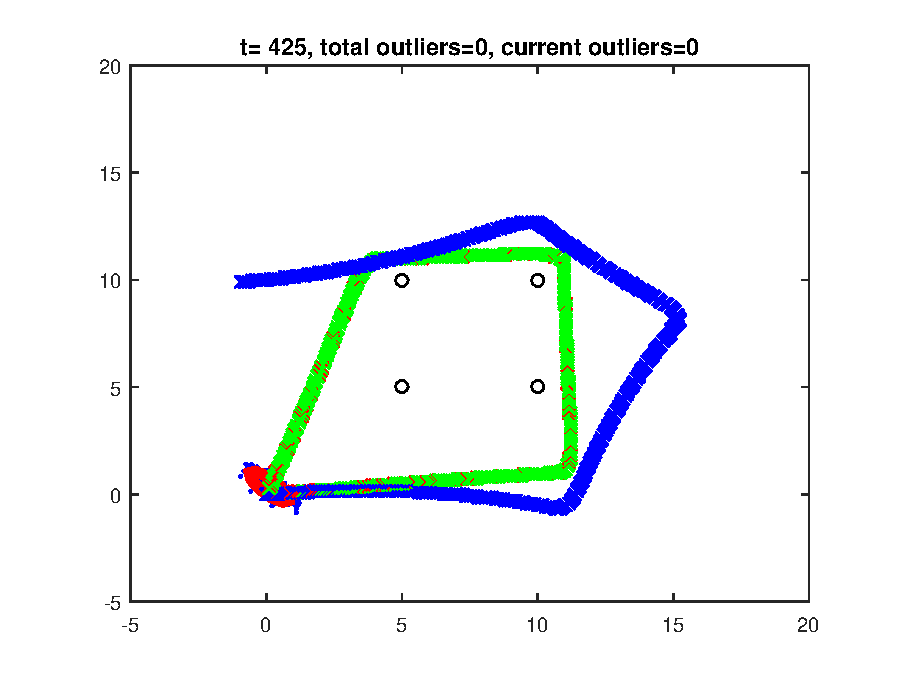
\includegraphics[width=0.6\textwidth]{sym2track1000}


\caption{Tracking task finished}
\label{fig:track}

\end{figure}

The different hypotheses appear in different parts of the map so in order to keep track of all of them some particles have to be initialized around them or they will not survive, that is why \texttt{part\_bound} has to be increased as this parameter controls the bounds of the area in the map where the particles are initialized randomly in the beginning. Figure \ref{fig:loc1000} shows the localisation task with 1000 particles. It can be seen how the multiple hypotheses that appear after 10 iterations disappear for 30 iterations and after 50 iterations only one remains, in this case the correct one.\\

\begin{figure}[htp]

\centering
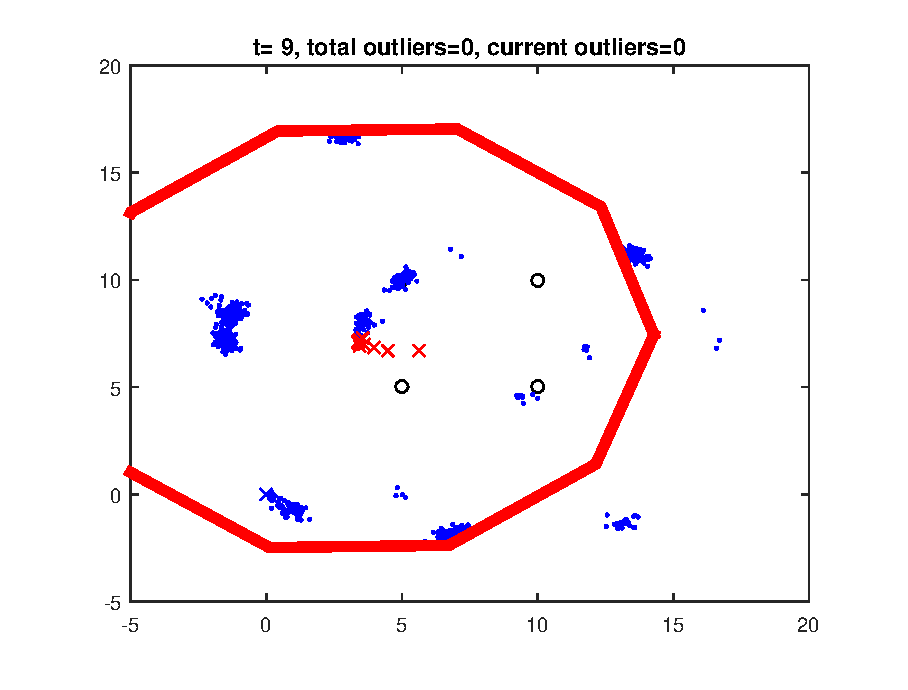
\includegraphics[width=.3\textwidth]{sym2loc1000_t10}\hfill
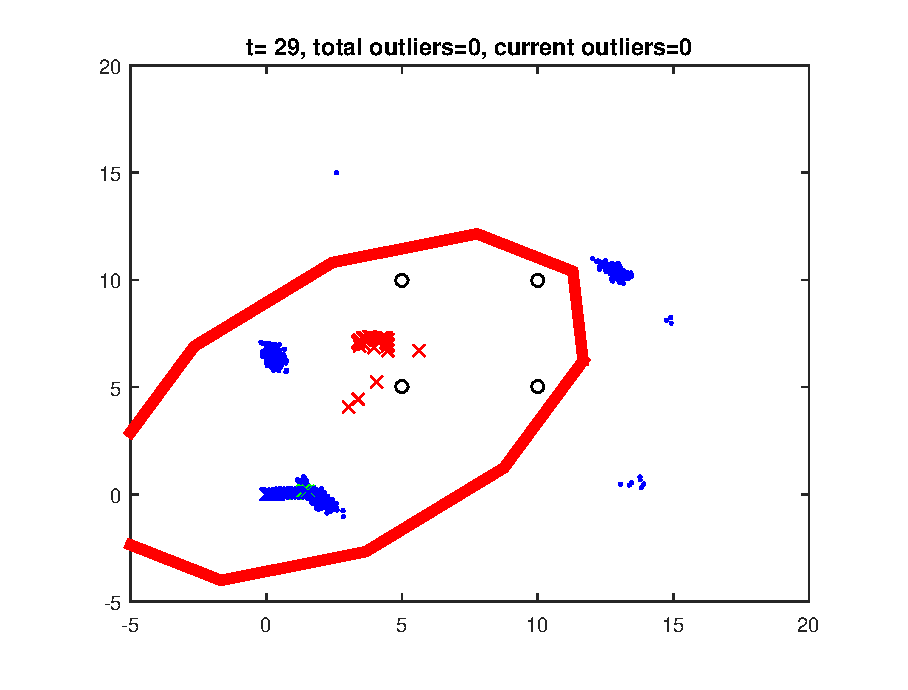
\includegraphics[width=.3\textwidth]{sym2loc1000_t30}\hfill
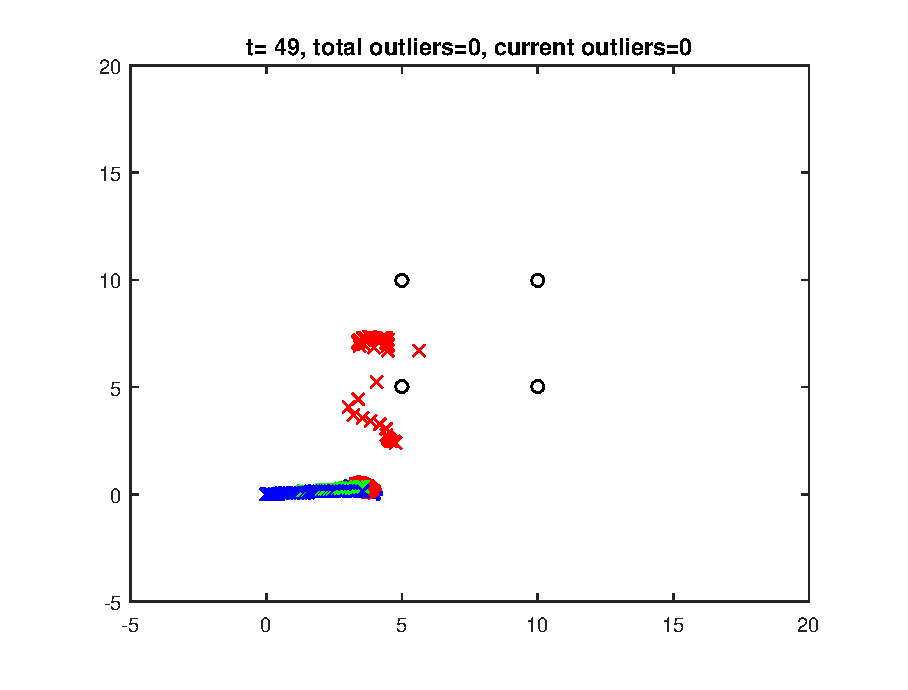
\includegraphics[width=.3\textwidth]{sym2loc1000_t50}

\caption{Localisation task for 1000 particles at t=10,30,50}
\label{fig:loc1000}

\end{figure}

Increasing the number of particles effectively makes the hypotheses to stay. In Figure \ref{fig:loc10000} the number of particles has been increased to 10000 and it can be seen how the 4 main hypotheses still appear after 50 iterations. This happens because now the number of particles with which to cover the areas with high likelihood is enough, before it was not so some areas where not covered, what is known as particle deprivation.\\

\begin{figure}[htp]

\centering
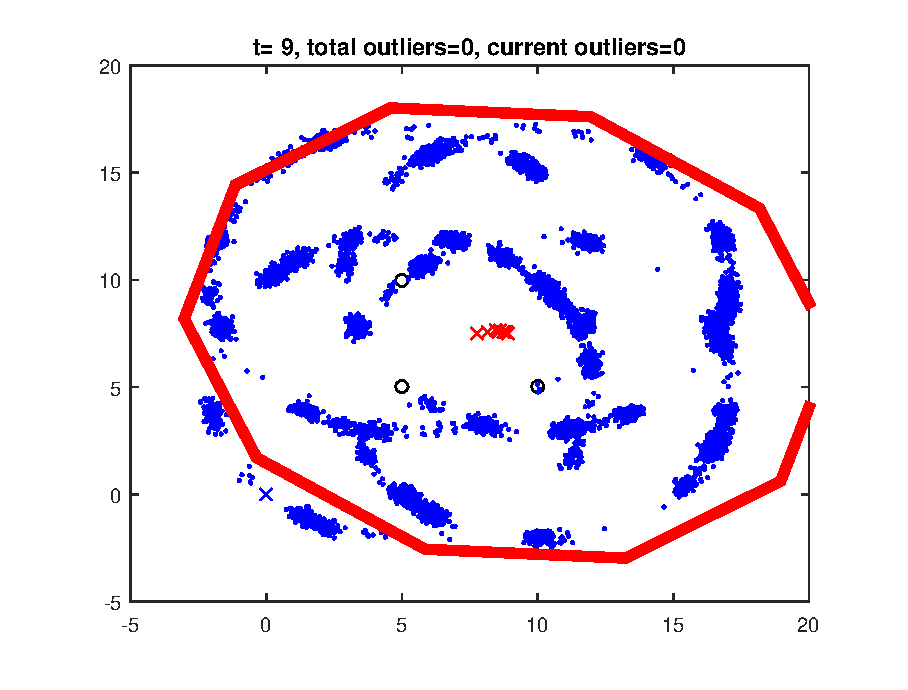
\includegraphics[width=.3\textwidth]{sym2loc10000_t10}\hfill
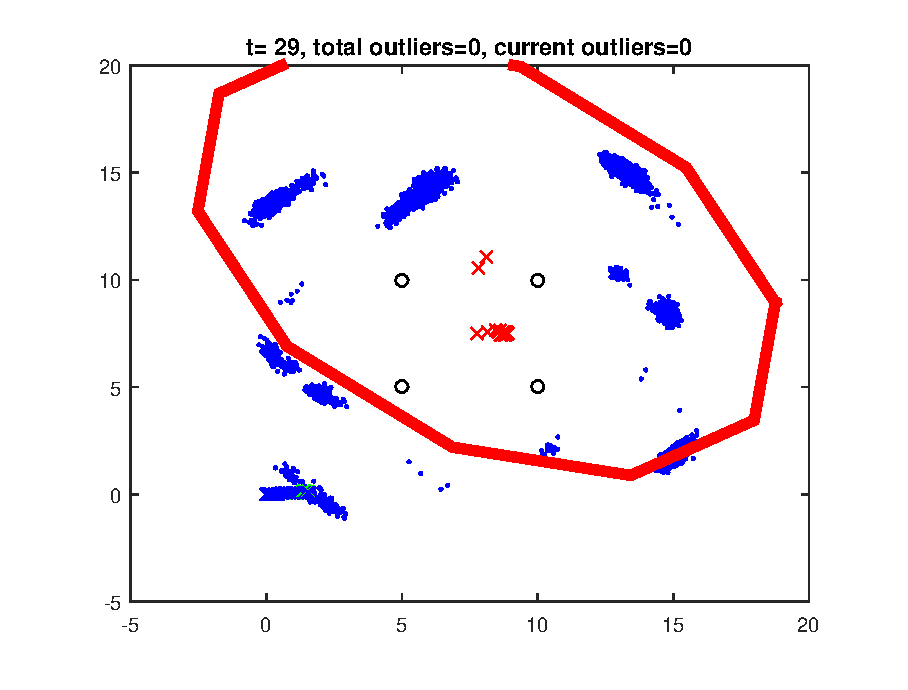
\includegraphics[width=.3\textwidth]{sym2loc10000_t30}\hfill
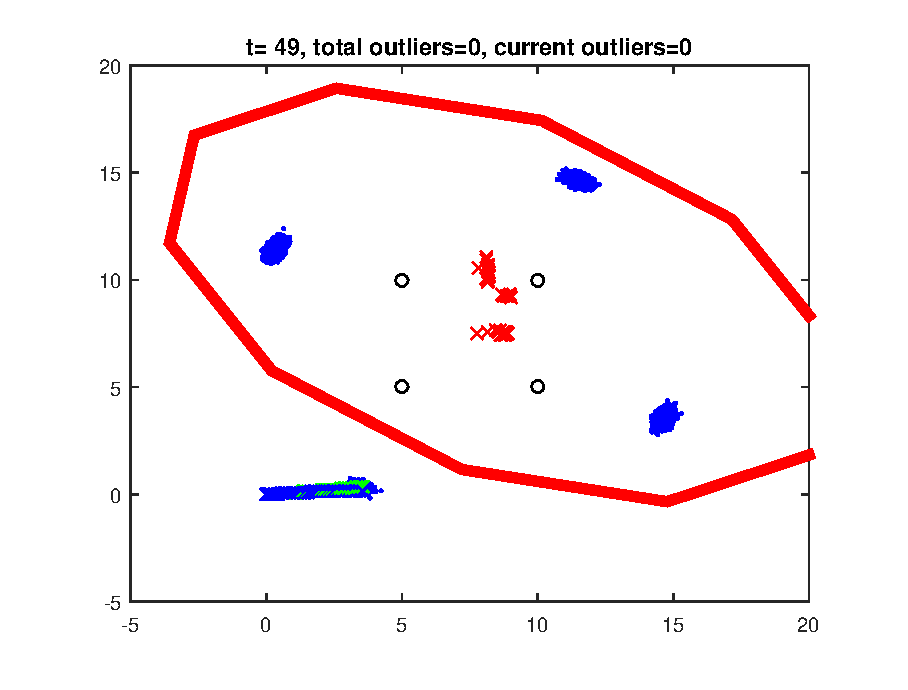
\includegraphics[width=.3\textwidth]{sym2loc10000_t50}

\caption{Localisation task for 10000 particles at t=10,30,50}
\label{fig:loc10000}

\end{figure}

This was using systematic re-sampling, using multinomial re-sampling the things change as with this method is more likely that particles with higher weights are chosen. Figure \ref{fig:locmulti} shows that the multiple hypotheses disappear even faster so it preserves them worse.\\

\begin{figure}[htp]

\centering
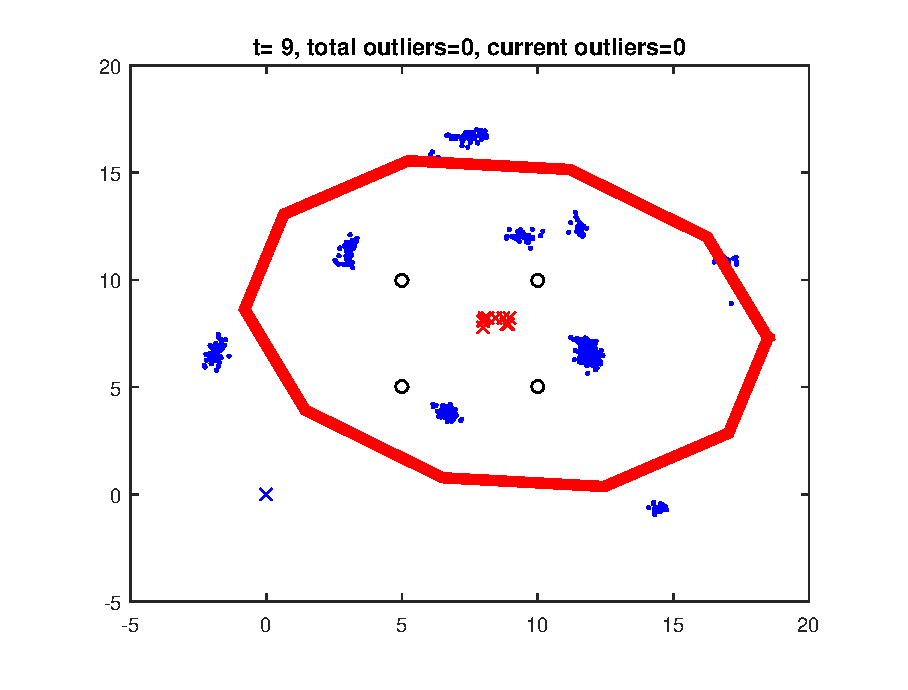
\includegraphics[width=.3\textwidth]{sym2loc1000_t10_multi}\hfill
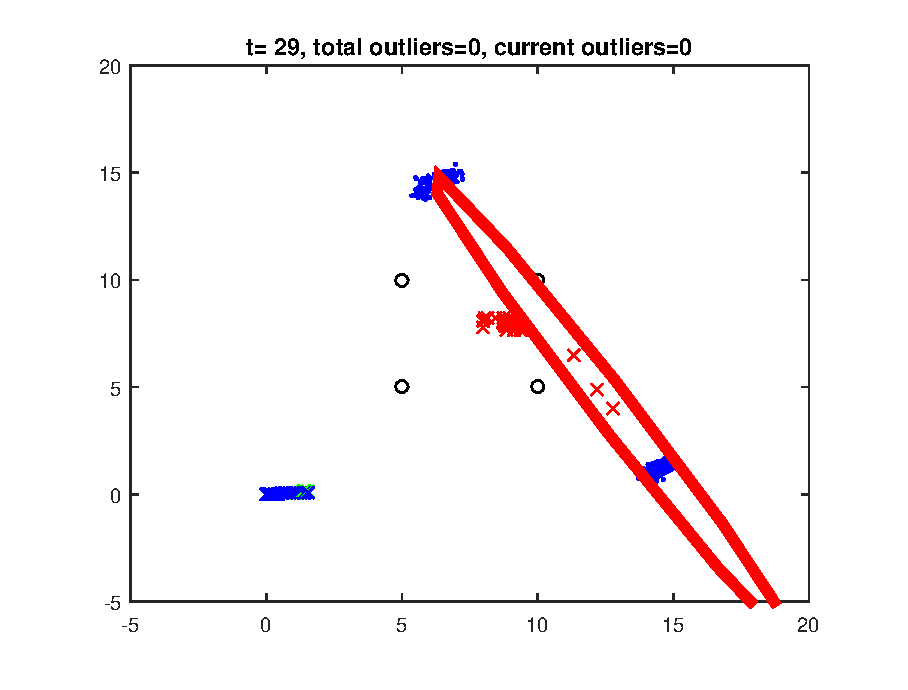
\includegraphics[width=.3\textwidth]{sym2loc1000_t30_multi}\hfill
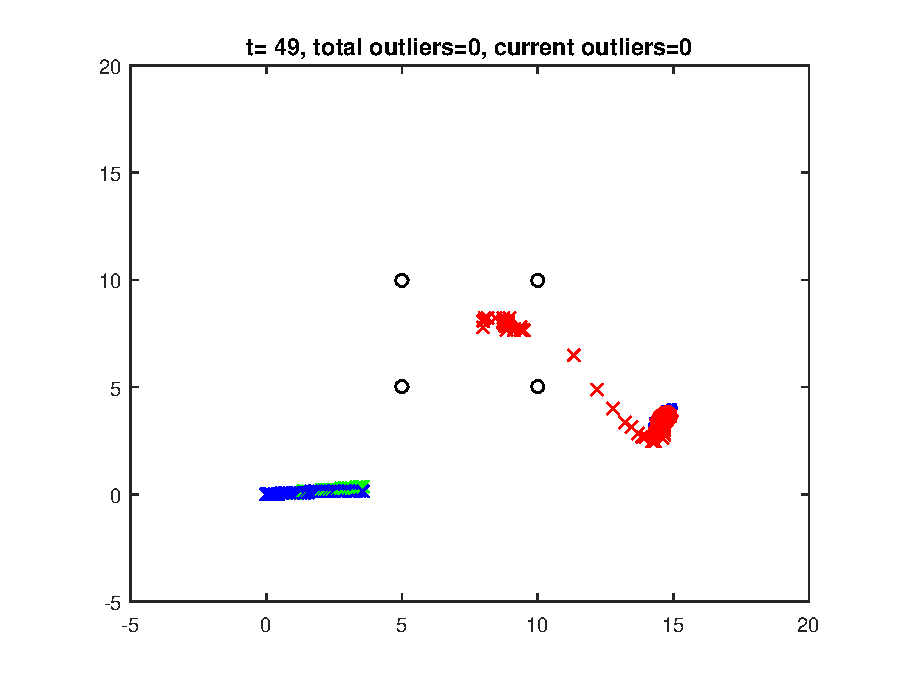
\includegraphics[width=.3\textwidth]{sym2loc1000_t50_multi}

\caption{Localisation task for 1000 particles at t=10,30,50 using multinomial re-sampling}
\label{fig:locmulti}

\end{figure}

Changing the measurement noise models also affects the hypotheses preservation. Figure \ref{fig:lochn} shows the results for stronger measurement noise and Figure \ref{fig:locln} for very weak noise. For stronger noise the hypotheses are better preserved although are more spread, for weaker noise the hypotheses disappear fast and in this case actually converge to an incorrect one.

\begin{figure}[htp]

\centering
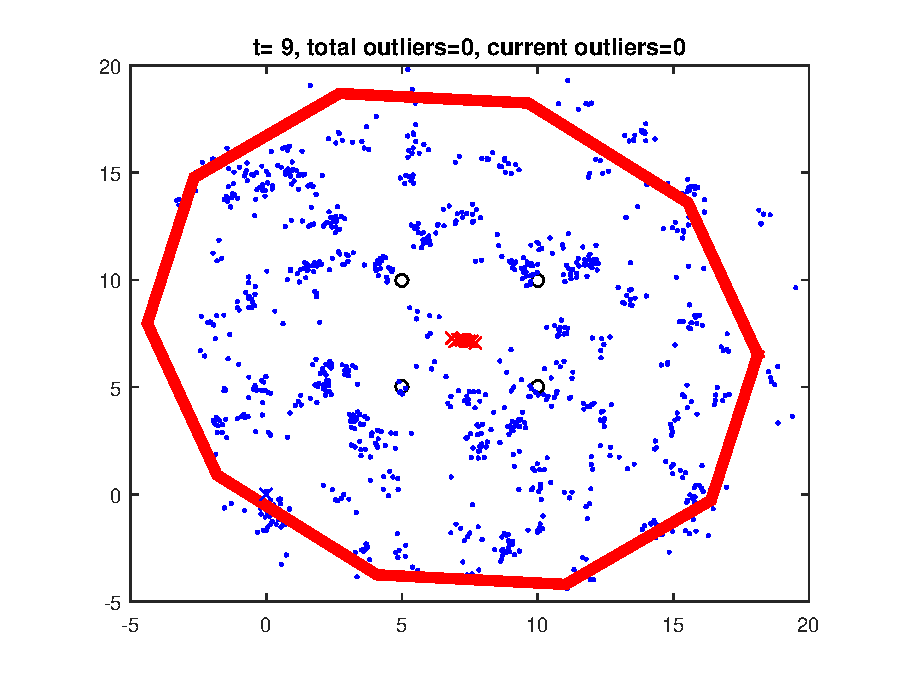
\includegraphics[width=.3\textwidth]{sym2loc1000_t10_highnoise}\hfill
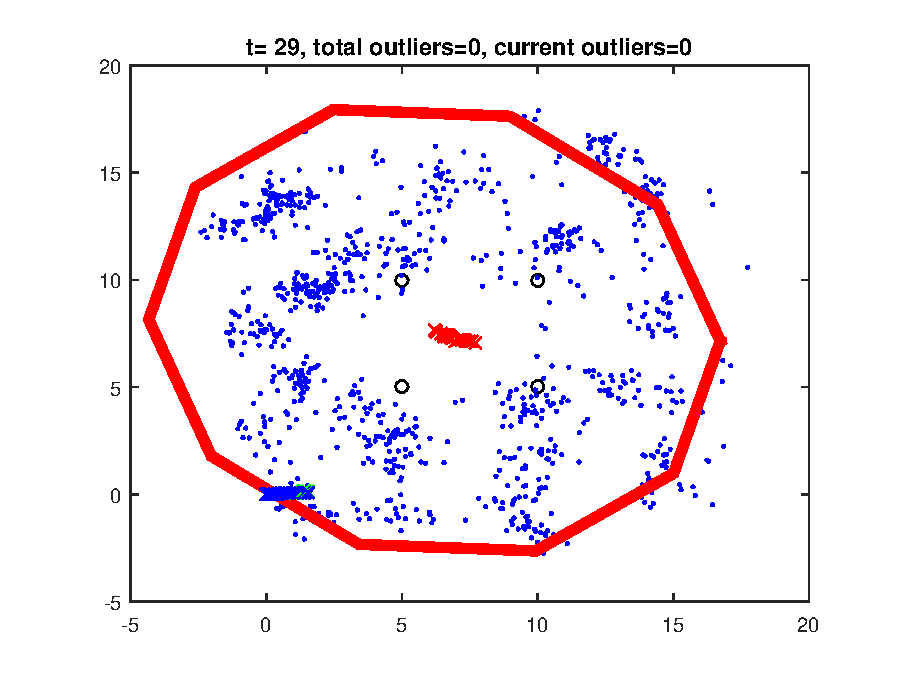
\includegraphics[width=.3\textwidth]{sym2loc1000_t30_highnoise}\hfill
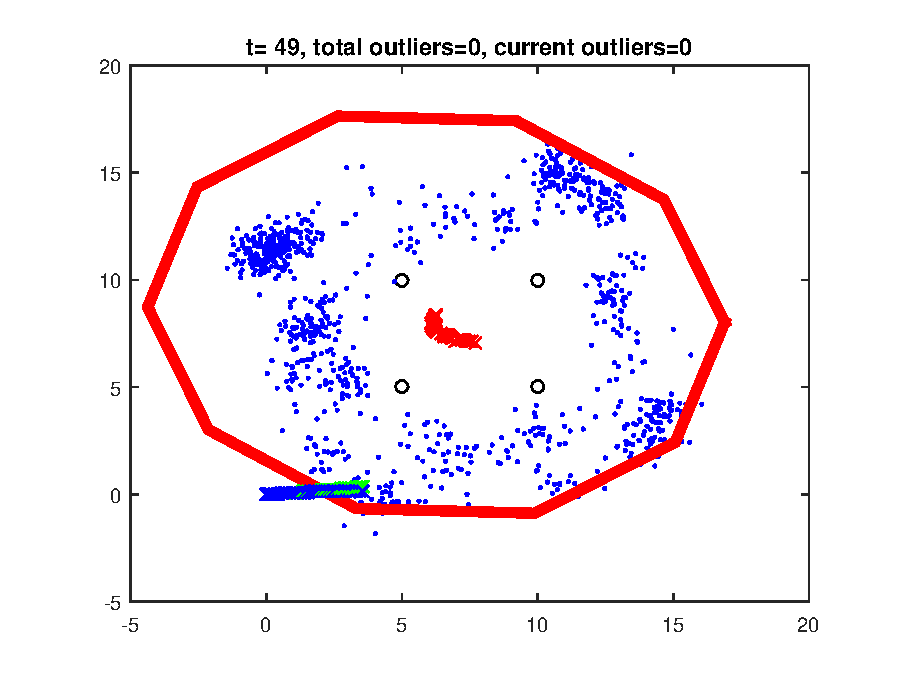
\includegraphics[width=.3\textwidth]{sym2loc1000_t50_highnoise}

\caption{Localisation task for 1000 particles at t=10,30,50 with Q multiplied by 100}
\label{fig:lochn}

\end{figure}
\begin{figure}[htp]

\centering
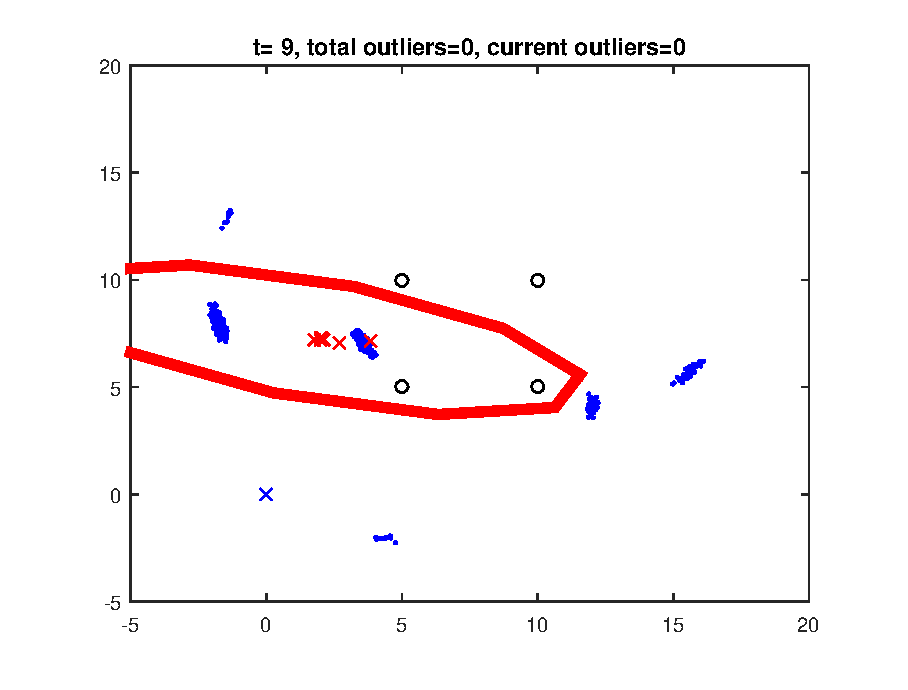
\includegraphics[width=.3\textwidth]{sym2loc1000_t10_lownoise}\hfill
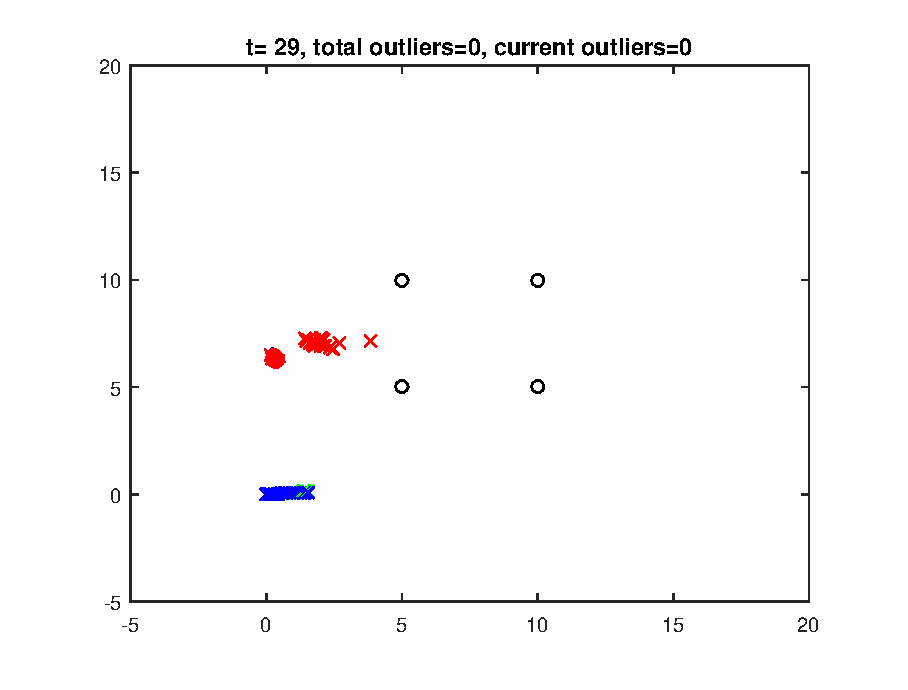
\includegraphics[width=.3\textwidth]{sym2loc1000_t30_lownoise}\hfill
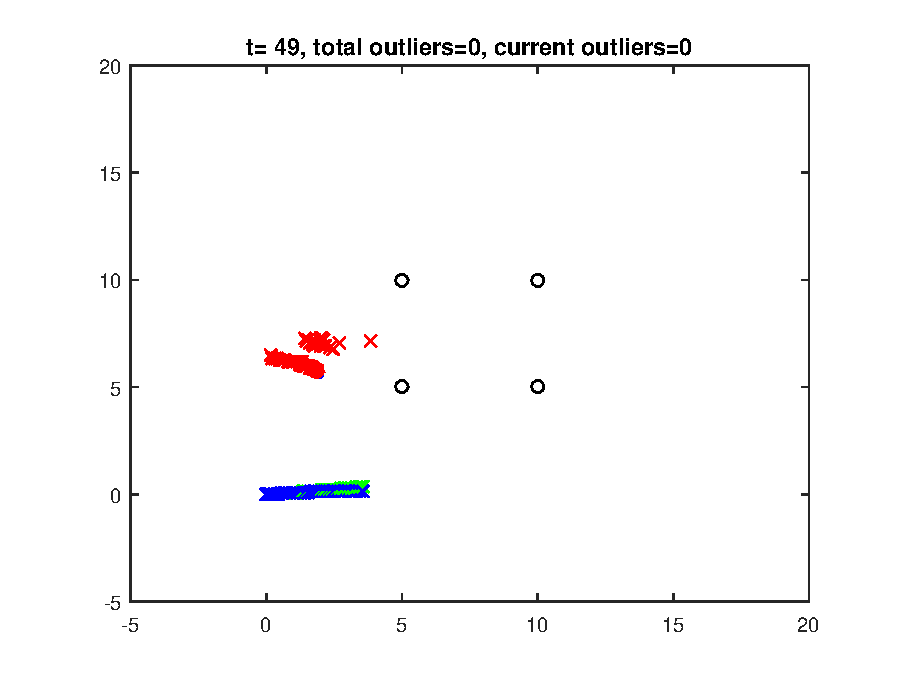
\includegraphics[width=.3\textwidth]{sym2loc1000_t50_lownoise}

\caption{Localisation task for 1000 particles at t=10,30,50 with Q divided by 10.}
\label{fig:locln}

\end{figure}

\subsubsection{\texttt{map\_sym3+so\_sym3\_nk}}

The results for the second map are shown in \ref{fig:loc3}. The first image to the left shows the filter with two different hypotheses before measuring the landmark breaking the symmetry. The second image instants after, in which the erroneous hypothesis has disappeared and the particle filter has converged to the correct hypothesis. The third image shows the completed localisation task. It can be seen how in the lower part the particle filter loses track of the correct position due to the lack of measurements in the area, but soon recovers when a new measurement is available.
\begin{figure}[htp]

\centering
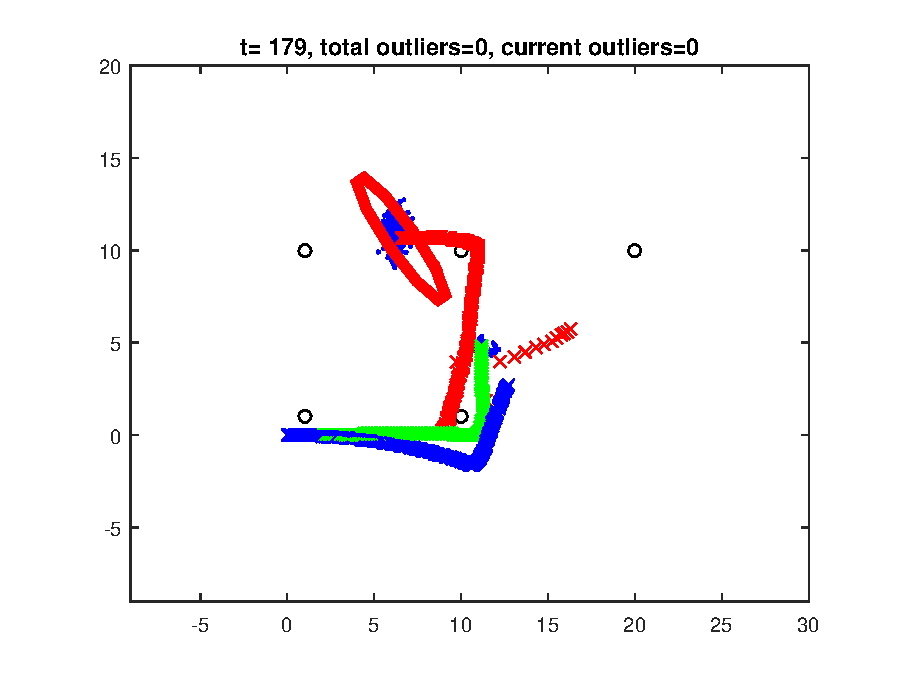
\includegraphics[width=.3\textwidth]{sym3loc1000_t179}\hfill
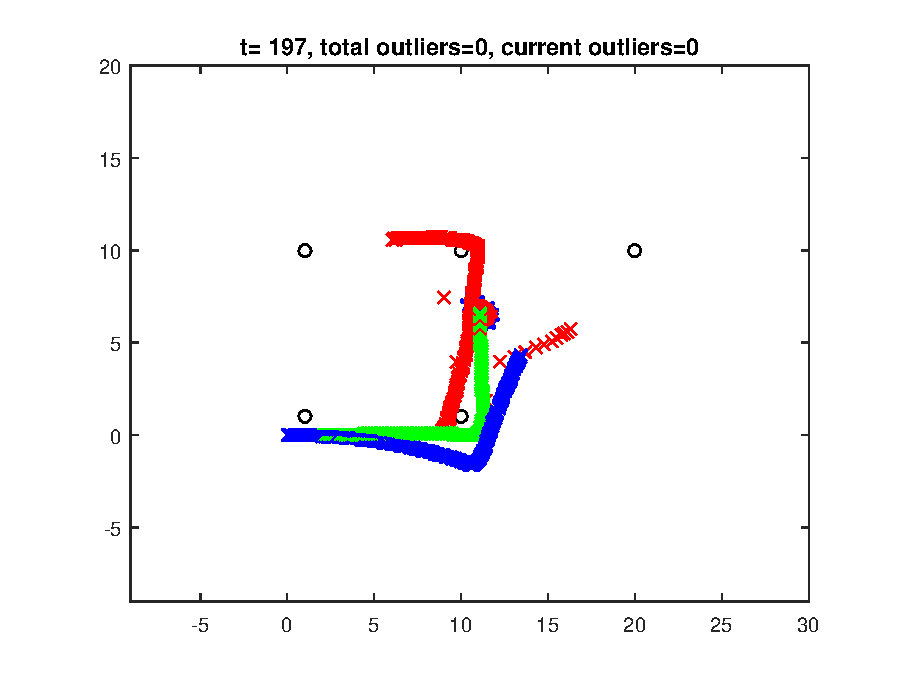
\includegraphics[width=.3\textwidth]{sym3loc1000_t197}\hfill
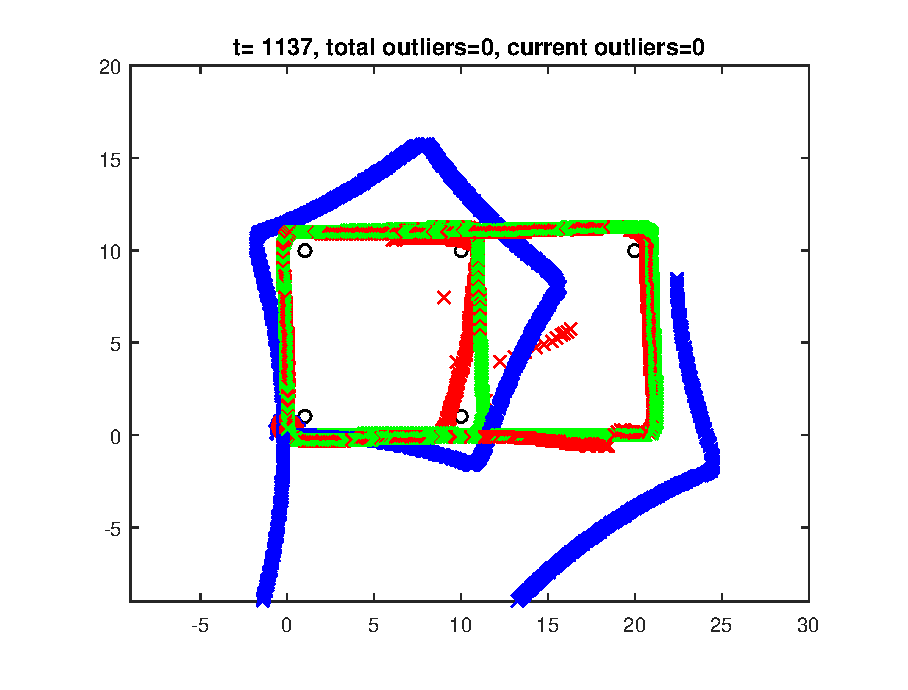
\includegraphics[width=.3\textwidth]{sym3loc1000_end}

\caption{Localisation task for 1000 particles with the map \texttt{map\_sym3}}
\label{fig:loc3}

\end{figure}





\end{document}